%%
%% GAC: When Smaller Is Slower — Dimensional Misalignment in Compressed LLMs
%% Target: EuroMLSys 2026 (SIGPLAN format, 6 pages excluding references)
%%

\documentclass[sigplan,10pt,nonacm]{acmart}

%% Remove ACM-specific elements for submission
\settopmatter{printacmref=false,authorsperrow=5}
\renewcommand\footnotetextcopyrightpermission[1]{}
\pagestyle{plain}

%% Packages
\usepackage{booktabs}
\usepackage{subcaption}
\usepackage{xcolor}
\usepackage{graphicx}
\usepackage{tikz}
\usetikzlibrary{positioning,decorations.pathreplacing,fit,backgrounds}
\usepackage{placeins}
\usepackage{colortbl}
\usepackage{enumitem}
\usepackage{algorithm}
\usepackage{algpseudocode}
\hfuzz=0pt  % Strict: report ALL overfull boxes

%% Compact spacing
\setlength{\textfloatsep}{8pt plus 2pt minus 2pt}
\setlength{\floatsep}{8pt plus 2pt minus 2pt}
\setlength{\intextsep}{6pt plus 2pt minus 2pt}
\setlength{\abovecaptionskip}{4pt}
\setlength{\belowcaptionskip}{2pt}

%% Colors matching slides
\definecolor{cblue}{RGB}{55,131,187}
\definecolor{cred}{RGB}{211,63,73}
\definecolor{cgreen}{RGB}{56,158,92}
\definecolor{corange}{RGB}{230,159,0}

%% Title
\title{Why Smaller Is Slower?\\ Dimensional Misalignment in Compressed LLMs}

%% Authors
\author{Jihao Xin}
\affiliation{
  \institution{KAUST}
  \country{Saudi Arabia}
}

\author{Tian Lyu}
\affiliation{
  \institution{KAUST}
  \country{Saudi Arabia}
}

\author{Qilong Pan}
\affiliation{
  \institution{HUMAIN AI}
  \country{Saudi Arabia}
}

\author{Kesen Wang}
\affiliation{
  \institution{HUMAIN AI}
  \country{Saudi Arabia}
}

\author{Marco Canini}
\affiliation{
  \institution{KAUST}
  \country{Saudi Arabia}
}

\begin{abstract}
Post-training compression reduces LLM parameter counts but often produces irregular tensor dimensions that degrade GPU performance---a phenomenon we call \emph{dimensional misalignment}.
We present a full-stack analysis of this effect, identifying root causes at three levels: framework (PyTorch backend dispatch), library (cuBLAS kernel selection), and hardware (TensorCore and memory alignment).
We propose \textbf{GAC} (GPU-Aligned Compression), a general framework that wraps any compressor and selects GPU-Aligned dimensions via multi-choice knapsack optimization.
On Llama-3-8B with two representative compressors---ASVD (SVD factorization) and LLM-Pruner (structured pruning)---GAC achieves 100\% dimension alignment with up to 1.5$\times$ speedup while preserving model quality.
\end{abstract}

\keywords{LLM Compression, GPU Optimization}

\begin{document}

\maketitle


%% ===========================================
%% 1. INTRODUCTION
%% ===========================================
\section{Introduction}
\label{sec:intro}

Large Language Models (LLMs) achieve strong capabilities but their scale poses deployment challenges~\cite{llama3}.
Post-training compression reduces model size which can be categorized into three categories: \emph{quantization} (reduced precision)~\cite{gptq,awq}, \emph{sparsification} (zeroing weights)~\cite{sparsegpt,wanda}, and \emph{dimension reduction} (low-rank factorization, structured pruning, KV cache eviction)~\cite{asvd,palu,llmpruner,h2o,pyramidkv}.
We focus on \textbf{dimension reduction}: it alters the tensor shapes that feed the dominant inference operators, which often produce \emph{irregular} dimensions (e.g., reduced rank from 128 to 107), which is inefficient in GPU's execution, and leads to a counterintuitive outcome: \emph{compressed models with \textbf{smaller} parameters can run \textbf{slower} than uncompressed models}. We term this \textbf{dimensional misalignment}.
We summarize three classes of compression algorithms that lead to dimensional misalignment: \textbf{(i)}~low-rank factorization (decomposing weight matrices into two smaller matrices $W \approx A \cdot B$, truncating inner dimension),~\cite{asvd,palu,svdllm2024}; \textbf{(ii)}~structured pruning (removing neurons or heads, reducing output dimension),~\cite{llmpruner,sparsegpt,wanda}; \textbf{(iii)}~token eviction (dropping or compressing keys/values, reducing effective sequence length),~\cite{h2o,pyramidkv}.

Existing compression methods predominantly trade off \emph{size and accuracy}: given a compression ratio, they maximize preserved accuracy while ignoring how chosen dimensions interact with hardware.
We propose \textbf{GAC} (GPU-Aligned Compression), a new compression \emph{paradigm} that imposes hardware alignment constraints on top of existing dimension-reducing compressors: it wraps any such compressor and selects hardware-aligned dimensions under the same parameter budget, restoring speed without changing the compressor's accuracy-oriented design.

\noindent \textbf{Contributions.}\\
\textbf{(1)}~We identify the \emph{dimensional misalignment} problem (\S\ref{sec:misalignment}).\\
\textbf{(2)}~We conduct a systematic full-stack analysis (\S\ref{sec:analysis}).\\
\textbf{(3)}~GAC formalizes the dimension selection as a constrained optimization with a dynamic programming solver (\S\ref{sec:gac}).\\
\textbf{(4)}~Preliminary evaluation on Llama-3-8B shows up to 1.5$\times$ speedup (\S\ref{sec:eval}).


%% ===========================================
%% 2. DIMENSIONAL MISALIGNMENT
%% ===========================================
\section{Motivation: Dimensional Misalignment}
\label{sec:misalignment}
\begin{figure*}[t]
  \centering
  \includegraphics[width=\textwidth]{figures/scatter_1x4_meta_llama_3_8b_instruct_r0.8.pdf}
  \caption{Llama-3-8B at $\rho=20\%$. Shape: $\circ{=}$Q Head, $\square{=}$K Head, $\triangle{=}$V Head; color: \textcolor{cgreen}{green}=8-aligned, \textcolor{cred}{red}=misaligned.}
  \label{fig:dim_scatter}
  \vspace{-0.3cm}
  \end{figure*}


Existing LLM compression aims to preserve accuracy under a given compression ratio $\rho$.
Formally, given the set of pretrained parameters $\mathcal{W}$, we seek a compressed set $\mathcal{W}'$ that minimizes expected loss subject to the size constraint:
\begin{equation}
\min_{\mathcal{W}'} \; \mathbb{E}_{(x,y)\sim\mathcal{D}}[\mathcal{L}(\mathcal{W}'; x, y)] \quad \text{s.t.} \quad 1-|\mathcal{W}'|/|\mathcal{W}| \leq \rho.
\label{eq:compression_target}
\end{equation}
Here $\mathcal{D}$ is the data distribution, $\mathcal{L}$ is the loss, $|\mathcal{W}'|$ and $|\mathcal{W}|$ denote total parameter counts. We denote $B = (1-\rho)|\mathcal{W}|$ as the parameter budget.

Different parameters have different compression sensitivities, e.g., early and late layers are often more critical than middle layers---so budget cannot be allocated uniformly.
Existing methods proceed in two steps.
First, for each parameter $W_i$, compute an \textbf{importance score} $s_i$ using a proxy (Table~\ref{tab:importance_scores}); a higher $s_i$ reflects higher sensitivity thus should retain more parameters in $W_i$.
Second, allocate the budget $B$ by assigning each $W_i$ a dimension $d_i$ thus that more important $W_i$ receive larger $d_i$:
\begin{equation}
\{d_i\} = \arg\max_{\{d_i\}} \sum_i s_i \cdot |W_i| \quad \text{s.t.} \quad |\mathcal{W}'| \leq B, \quad d_i \geq 0.
\label{eq:budget_allocation}
\end{equation}
Here $d_i$ is the compressed dimension (e.g., inner rank or output width, varies by compression method), $|W_i|$ is the parameter count given dimension $d_i$, $|\mathcal{W}'| = \sum_i |W_i|$ is the total parameter count of the compressed model, and $B$ is the parameter budget.
Because $s_i$ and the optimum $\{d_i\}$ are continuous, the resulting dimensions are typically \emph{irregular} (e.g., 107, 108, 109) and often violate GPU alignment requirements (e.g.\ $d \bmod 8 = 0$), triggering backend fallbacks and kernel switches that erase the expected speedup from fewer parameters and FLOPs.

We demonstrate the dimensional misalignment problem with a real-world example: PaLU~\cite{palu}.
We use \textbf{8-alignment} ($d \bmod 8 = 0$) as an example of alignment constraints. When dimensions are not 8-aligned, latency can increase by up to 90\% (Figure~\ref{fig:sdpa_latency}); we detail this analysis in \S\ref{sec:analysis}.
Figure~\ref{fig:palu_dist} shows that a large fraction of layers end up misaligned (e.g., 78\% in this setup).
For generality, we summarize the mainstream importance score proxies into four categories (Table~\ref{tab:importance_scores}).
We empirically measure unconstrained dimension allocation on Llama-3-8B at $\rho=20\%$ with all four proxies, Figure~\ref{fig:dim_scatter} demonstrates the dimensional misalignment consistently occurs across different methods.
\begin{figure}[t]
\centering
\includegraphics[width=\columnwidth]{figures/fig3_palu_dist.png}
\caption{Llama-3-8B after PaLU compression at $\rho=20\%$.}
\label{fig:palu_dist}
\end{figure}

\begin{table}[t]
\centering
\caption{Mainstream importance score for budget allocation.}
\label{tab:importance_scores}
\small
\setlength{\tabcolsep}{2.5pt}
\begin{tabular}{@{}llll@{}}
\toprule
\textbf{Method} & \textbf{Score} & \textbf{Intuition} & \textbf{Works} \\
\midrule
Magnitude & $\|W_i\|_F$ & Weight norm & SVD-LLM~\cite{svdllm2024} \\
Activation & $\|X_i\|_F$ & Input mag.\  & ASVD~\cite{asvd} \\
Gradient & $\left|\frac{\partial \mathcal{L}}{\partial h_i} \cdot h_i\right|$ & Taylor exp.\  & \cite{taylor_pruning} \\
Fisher & $\mathrm{tr}(\mathbf{F}_i)$ & Loss curvature & PaLU \cite{palu} \\
\bottomrule
\end{tabular}
\end{table}


%% ===========================================
%% 3. FULL-STACK ANALYSIS
%% ===========================================

\section{Full-Stack Analysis}
\label{sec:analysis}
We analyze where and why dimensional misalignment causes slowdowns on an NVIDIA A100-80GB with PyTorch 2.9.1, CUDA 12.8, FP16.
Latency is measured with CUDA events (50 warmup, 200 measurement iterations, 3 trials).
Root causes fall into three layers (Figure~\ref{fig:fullstack_overview}): Framework, Library, and Hardware. We detail each layer in the following subsections.
\begin{figure}[t]
  \centering
  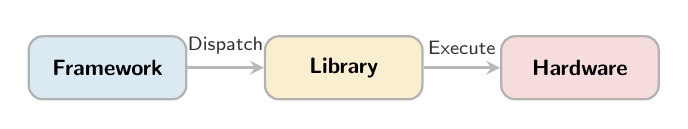
\begin{tikzpicture}[
      box/.style={draw=gray!60, rounded corners=5pt, minimum width=2.0cm, minimum height=0.8cm,
                  line width=0.8pt, font=\sffamily\footnotesize\bfseries, align=center, inner sep=4pt},
      >=stealth, arrow/.style={->, line width=1.2pt, gray!55},
      lbl/.style={font=\sffamily\scriptsize, text=gray!40!black, above=1pt}
    ]
    \node[box, fill=cblue!18] (fw) at (0,0) {Framework};
    \node[box, fill=corange!18] (lib) at (3.0,0) {Library};
    \node[box, fill=cred!18] (hw) at (6.0,0) {Hardware};
    \draw[arrow] (fw) -- (lib) node[midway, lbl] {Dispatch};
    \draw[arrow] (lib) -- (hw) node[midway, lbl] {Execute};
  \end{tikzpicture}
  \caption{Hierarchical Analysis.}
  \label{fig:fullstack_overview}
  \end{figure}

\subsection{Framework Layer}
\label{sec:framework}
Existing DL frameworks such as PyTorch and TensorFlow dispatch an operation to different backends.
For example, a matrix multiply \texttt{A@B} in PyTorch may run via cuBLAS or via a Triton kernel depending on the shape and hardware, where the dispatching mechanism is hidden from the user.
In this section, we exemplify this issue via PyTorch's \textbf{SDPA} (Scaled Dot-Product Attention), the core attention mechanism:
\begin{equation}
\mathrm{Attention}(Q,K,V) = \mathrm{softmax}(Q K^\top / \sqrt{d_k}) V
\end{equation}
where $Q$, $K$, $V$ are the query, key, and value matrices and $d_k$ is the per-head dimension.
When one calls the SDPA API \footnote{\texttt{torch.nn.functional.scaled\_dot\_product\_attention(Q, K, V)}} , PyTorch may select an optimized implementation (e.g., FlashAttention) or fall back to a naive eager implementation (the ``Math'' backend).

We measured SDPA latency with inputs $Q,K,V$ of shape $(B, S, H, d)$: batch $B{=}4$, sequence length $S{=}2048$, number of heads $H{=}32$, and we sweep the per-head dimension $d$ from 64 to 256 (full sweep details in Appendix~\ref{app:fa2_templates}).
We observed a staircase pattern (Figure~\ref{fig:sdpa_latency}).
First, multiples of 8 are faster: e.g., $d{=}129$ incurs $\sim$90\% higher latency than $d{=}128$.
Profiling shows that PyTorch uses FlashAttention only when $d \bmod 8 = 0$; otherwise it falls back to the Math kernel.
Second, among 8-aligned dimensions, $d \bmod 32 = 0$ forms another performance boundary: FlashAttention-2 uses dimension-specific templates, with tile sizes changing every 32 dimensions.
In the figure, alternating background shades denote template regions; labels such as ``$t{=}96$, $128{\times}64$'' indicate the template size $t$ and the $B_r {\times} B_c$ tile shape for that region.
\begin{figure}[t]
  \centering
  \includegraphics[width=\columnwidth]{figures/fig2_sdpa_latency.pdf}
  \caption{PyTorch SDPA latency across dimensions.}
  \label{fig:sdpa_latency}
  \end{figure}


\subsection{Library Layer}
\label{sec:library}

Linear algebra is dispatched to libraries (e.g., cuBLAS), where the same GEMM can be served by different kernels depending on dimensions.
We examine this via GEMM $C {=} A {\cdot} B$ with $A \in \mathbb{R}^{M \times K}$ and $B \in \mathbb{R}^{K \times N}$.
We measured GeMM latency with two of $(M, N, K)$ fixed at typical LLM sizes ($M{=}N{=}2048$, $K{=}128$) and the third dimension swept from 50\% to 100\%.
Figure~\ref{fig:gemm_alignment} shows the results.
First, $K$ and $N$ exhibit a clear alignment effect: when the swept dimension satisfies $d \bmod 8 = 0$, latency is lower (e.g., $K$ aligned $\sim$20\,$\mu$s vs.\ misaligned 22--26\,$\mu$s, up to 30\% penalty).
Second, $M$ and $N$ show \emph{kernel-switching cliffs}: at certain boundaries (e.g., $M{=}1728 \to 1729$), latency jumps (e.g., $\sim$30\%).
We profiled with Nsight Compute to explain this: when $d \bmod 8 = 0$, cuBLAS invokes its native optimized kernel; otherwise it uses a CUTLASS-generated kernel, which is further divided into align2 (fetching 2 elements at a time) or align1.
Table~\ref{tab:cublas_tiers} summarizes the three tiers.
GeMV ($M{=}1$) exhibits a similar but smaller penalty (${\sim}$12\% on $K$, ${\sim}$4\% on $N$; Appendix~\ref{app:gemv}), consistent with GeMV being memory-bound rather than compute-bound.
\begin{table}[t]
\centering
\caption{cuBLAS GEMM kernel tiers (Nsight Compute).}
\label{tab:cublas_tiers}
\small
\setlength{\tabcolsep}{2pt}
\resizebox{\columnwidth}{!}{%
\begin{tabular}{@{}clll@{}}
\toprule
\textbf{Tier} & \textbf{Condition} & \textbf{Kernel} & \textbf{MMA Instr.} \\
\midrule
\rowcolor{cgreen!10} 1 & $d \bmod 8 = 0$ & cuBLAS-native sm80 & \texttt{mma.m16n8k16} \\
\rowcolor{corange!10} 2 & $d \bmod 2 = 0$ & CUTLASS sm80 align2 & \texttt{mma.m16n8k16} \\
\rowcolor{cred!10} 3 & odd & CUTLASS sm75 align1 & \texttt{mma.m16n8k8} \\
\bottomrule
\end{tabular}%
}
\end{table}

\begin{figure*}[t]
\centering
\includegraphics[width=\textwidth]{figures/fig_gemm_alignment.pdf}
\caption{GeMM latency with dimension sweep.}
\label{fig:gemm_alignment}
\end{figure*}

\subsection{Hardware Layer}
\label{sec:hardware}
Beyond framework and library dispatch, misaligned dimensions also cause inefficiency from the hardware level.
We use Nsight Compute profiling to isolate two mechanisms.
\textbf{(1)~Tensor Core}: The A100 MMA instruction \texttt{mma.m16n8k16} processes tiles of $16{\times}8{\times}16$ fp16 elements; dimensions not divisible by these tile sizes leave partial tiles underutilized.
A throughput sweep near $K,N{=}4096$ confirms: aligned dimensions reach 160--175 TFLOPS while misaligned ones drop to 50--110 TFLOPS, with period-16 in $K$ and period-8 in $N$ matching the tile shape (Figure~\ref{fig:hw_alignment}a,b).
\textbf{(2)~Memory}: The A100 L2 cache operates in 32-byte sectors; for FP16 this requires $K \bmod 16 = 0$ for full utilization.
Misaligned accesses show ${\sim}$2$\times$ bandwidth loss in microbenchmarks (Figure~\ref{fig:hw_alignment}c).

\begin{figure*}[t]
\centering
\includegraphics[width=\textwidth]{figures/fig_hw_alignment.pdf}
\caption{Hardware-level alignment penalties (sweep near 4096): (a,b)~Tensor Core throughput, (c)~L2 cache bandwidth.}
\label{fig:hw_alignment}
\end{figure*}

\paragraph{Summary.} Table~\ref{tab:constraints} summarizes all constraints.
The minimum requirement across all layers is $d \bmod 8 = 0$; stricter alignment (mod~16, mod~32) yields further gains.
These penalties compound: a single misaligned dimension can trigger a backend fallback, a suboptimal kernel, and underutilized tiles simultaneously.

\begin{table}[t]
\centering
\caption{Full-stack alignment constraint summary.}
\label{tab:constraints}
\small
\setlength{\tabcolsep}{2.5pt}
\begin{tabular}{@{}lllr@{}}
\toprule
\textbf{Level} & \textbf{Mechanism} & \textbf{Constraint} & \textbf{Penalty} \\
\midrule
\rowcolor{cblue!8} Framework & SDPA backend & $d$\%$8{=}0$ & ${\sim}$90\% \\
\rowcolor{cblue!8} Framework & FA2 template & $d$\%$32{=}0$ & ${\sim}$30\% \\
\midrule
\rowcolor{corange!8} Library & cuBLAS GeMM & $K$/$N$\%$8{=}0$ & ${\sim}$90\% \\
\rowcolor{corange!8} Library & cuBLAS GeMV & $K$\%$8{=}0$ & ${\sim}$12\% \\
\midrule
\rowcolor{cred!8} Hardware & TC MMA & $K$\%16, $N$\%8 & ${\sim}$70\% \\
\rowcolor{cred!8} Hardware & L2 sectors & $K$\%$16{=}0$ & ${\sim}$50\% \\
\bottomrule
\end{tabular}
\end{table}

%% ===========================================
%% 4. GAC: ALIGNMENT-AWARE COMPRESSION
%% ===========================================
\section{GAC: GPU-Aligned Compression}
\label{sec:gac}

% fig_gac_framework.tex — GAC Framework Pipeline (TikZ)
% Usage: % fig_gac_framework.tex — GAC Framework Pipeline (TikZ)
% Usage: % fig_gac_framework.tex — GAC Framework Pipeline (TikZ)
% Usage: \input{figures/fig_gac_framework.tex}
\begin{figure*}[t]
\centering
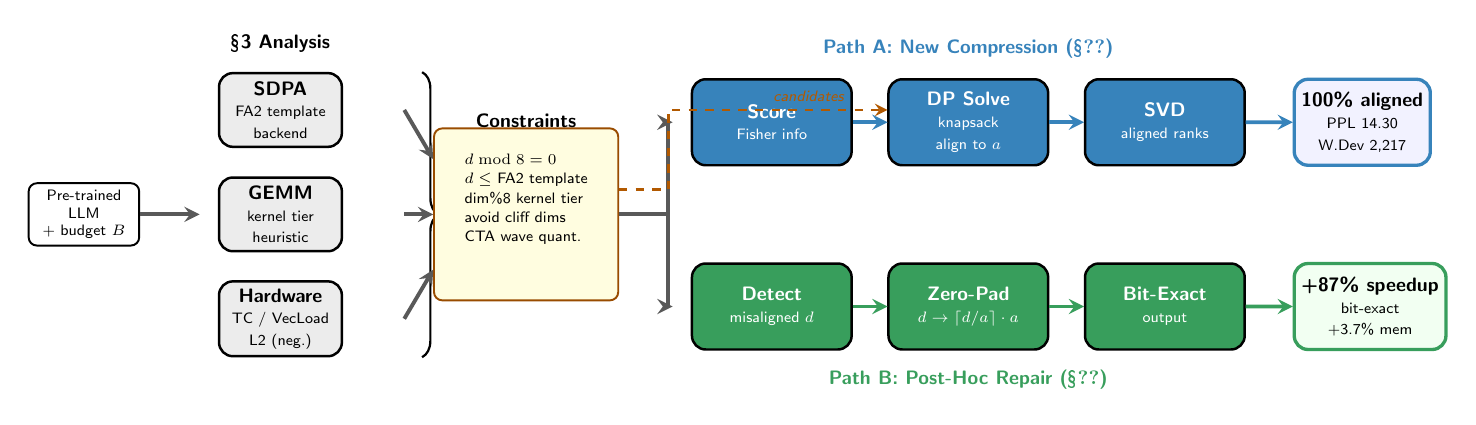
\begin{tikzpicture}[scale=0.78, every node/.style={scale=0.78},
    >=stealth,
    % Colors
    cblue/.style={fill={rgb,255:red,55;green,131;blue,187}},
    cred/.style={fill={rgb,255:red,211;green,63;blue,73}},
    cgreen/.style={fill={rgb,255:red,56;green,158;blue,92}},
    corange/.style={fill={rgb,255:red,230;green,159;blue,0}},
    cgray/.style={fill=gray!15},
    % Box styles
    phase/.style={draw, rounded corners=5pt, minimum width=2.4cm, minimum height=1.6cm,
                  line width=0.9pt, text=white, font=\sffamily\small, align=center},
    constraint/.style={draw, rounded corners=3pt, minimum width=2.0cm, minimum height=0.7cm,
                       line width=0.7pt, font=\sffamily\scriptsize, align=center,
                       fill=yellow!12, draw=orange!60!black},
    result/.style={draw, rounded corners=5pt, minimum width=2.2cm, minimum height=1.6cm,
                   line width=1.2pt, font=\sffamily\small, align=center},
    lbl/.style={font=\sffamily\small, align=center},
    arrow/.style={->, line width=1.4pt, color=gray!70!black},
    dasharrow/.style={->, line width=1.0pt, dashed, color=gray!50},
  ]

  % ===== LEFT: Analysis (§3) =====
  \node[phase, cgray, text=black, minimum width=2.0cm, minimum height=1.2cm]
    (sdpa) at (0, 1.2) {\textbf{SDPA}\\[-1pt]{\scriptsize FA2 template}\\[-1pt]{\scriptsize backend}};
  \node[phase, cgray, text=black, minimum width=2.0cm, minimum height=1.2cm]
    (gemm) at (0, -0.5) {\textbf{GEMM}\\[-1pt]{\scriptsize kernel tier}\\[-1pt]{\scriptsize heuristic}};
  \node[phase, cgray, text=black, minimum width=2.0cm, minimum height=1.2cm]
    (hw) at (0, -2.2) {\textbf{Hardware}\\[-1pt]{\scriptsize TC / VecLoad}\\[-1pt]{\scriptsize L2 (neg.)}};

  % Brace for analysis
  \node[above=0.15cm of sdpa, font=\sffamily\bfseries\small] {\S3 Analysis};
  \draw[decorate, decoration={brace, amplitude=6pt, raise=2pt}, line width=0.8pt]
    ([xshift=1.2cm]sdpa.north east) -- ([xshift=1.2cm]hw.south east);

  % ===== CENTER: Constraints =====
  \node[constraint, minimum width=3.0cm, minimum height=2.8cm]
    (constraints) at (4.0, -0.5) {};
  \node[above=-0.1cm of constraints.north, font=\sffamily\bfseries\small] {Constraints};
  \node[font=\sffamily\scriptsize, align=left, anchor=north] at ([yshift=-0.3cm]constraints.north) {
    $d \bmod 8 = 0$\\[1pt]
    $d \leq$ FA2 template\\[1pt]
    dim\%8 kernel tier\\[1pt]
    avoid cliff dims\\[1pt]
    CTA wave quant.
  };

  % Arrows: analysis → constraints
  \draw[arrow] ([xshift=1.0cm]sdpa.east) -- ([yshift=0.9cm]constraints.west);
  \draw[arrow] ([xshift=1.0cm]gemm.east) -- (constraints.west);
  \draw[arrow] ([xshift=1.0cm]hw.east) -- ([yshift=-0.9cm]constraints.west);

  % ===== RIGHT: Two paths =====
  % Path A: GAC DP (new compression)
  \node[phase, cblue, minimum width=2.6cm, minimum height=1.4cm]
    (score) at (8.0, 1.0) {\textbf{Score}\\[-1pt]{\scriptsize Fisher info}};
  \node[phase, cblue, minimum width=2.6cm, minimum height=1.4cm]
    (dp) at (11.2, 1.0) {\textbf{DP Solve}\\[-1pt]{\scriptsize knapsack}\\[-1pt]{\scriptsize align to $a$}};
  \node[phase, cblue, minimum width=2.6cm, minimum height=1.4cm]
    (svd) at (14.4, 1.0) {\textbf{SVD}\\[-1pt]{\scriptsize aligned ranks}};

  % Path B: Dimension Repair (existing model)
  \node[phase, cgreen, minimum width=2.6cm, minimum height=1.4cm]
    (detect) at (8.0, -2.0) {\textbf{Detect}\\[-1pt]{\scriptsize misaligned $d$}};
  \node[phase, cgreen, minimum width=2.6cm, minimum height=1.4cm]
    (pad) at (11.2, -2.0) {\textbf{Zero-Pad}\\[-1pt]{\scriptsize $d \to \lceil d/a\rceil \cdot a$}};
  \node[phase, cgreen, minimum width=2.6cm, minimum height=1.4cm]
    (exact) at (14.4, -2.0) {\textbf{Bit-Exact}\\[-1pt]{\scriptsize output}};

  % Arrows within paths
  \draw[arrow, color={rgb,255:red,55;green,131;blue,187}] (score) -- (dp);
  \draw[arrow, color={rgb,255:red,55;green,131;blue,187}] (dp) -- (svd);
  \draw[arrow, color={rgb,255:red,56;green,158;blue,92}] (detect) -- (pad);
  \draw[arrow, color={rgb,255:red,56;green,158;blue,92}] (pad) -- (exact);

  % Constraints → paths
  \draw[arrow] (constraints.east) -- ++(0.8,0) |- ([xshift=-0.3cm]score.west)
    node[pos=0.25, above, font=\sffamily\scriptsize\itshape] {};
  \draw[arrow] (constraints.east) -- ++(0.8,0) |- ([xshift=-0.3cm]detect.west);

  % Constraints feeds into DP
  \draw[dasharrow, color=orange!70!black]
    ([yshift=0.4cm]constraints.east) -- ++(0.8,0) |- ([yshift=0.2cm]dp.west)
    node[pos=0.82, above, font=\sffamily\scriptsize\itshape, text=orange!70!black] {candidates};

  % Path labels
  \node[above=0.15cm of dp, font=\sffamily\bfseries\small, text={rgb,255:red,55;green,131;blue,187}]
    {Path A: New Compression (\S\ref{sec:gac})};
  \node[below=0.15cm of pad, font=\sffamily\bfseries\small, text={rgb,255:red,56;green,158;blue,92}]
    {Path B: Post-Hoc Repair (\S\ref{sec:repair})};

  % Results on the right
  \node[result, fill=blue!5, draw={rgb,255:red,55;green,131;blue,187},
        right=0.6cm of svd, minimum height=1.4cm] (resA) {
    {\small\bfseries 100\% aligned}\\[-1pt]
    {\scriptsize PPL 14.30}\\[-1pt]
    {\scriptsize W.Dev 2{,}217}
  };
  \node[result, fill=green!5, draw={rgb,255:red,56;green,158;blue,92},
        right=0.6cm of exact, minimum height=1.4cm] (resB) {
    {\small\bfseries +87\% speedup}\\[-1pt]
    {\scriptsize bit-exact}\\[-1pt]
    {\scriptsize +3.7\% mem}
  };
  \draw[arrow, color={rgb,255:red,55;green,131;blue,187}] (svd) -- (resA);
  \draw[arrow, color={rgb,255:red,56;green,158;blue,92}] (exact) -- (resB);

  % Input on the left
  \node[draw, rounded corners=3pt, fill=white, line width=0.7pt,
        font=\sffamily\scriptsize, align=center, minimum width=1.8cm]
    (input) at (-3.2, -0.5) {Pre-trained\\LLM\\+ budget $B$};
  \draw[arrow] (input) -- ([xshift=-0.3cm]gemm.west |- input);

\end{tikzpicture}
\caption{\textbf{GAC framework overview.}
Analysis (\S\ref{sec:analysis}) extracts alignment constraints from three layers (SDPA, GEMM, hardware).
These constraints drive two complementary solutions:
\emph{Path~A}---alignment-aware rank allocation via multi-choice knapsack DP for new compression;
\emph{Path~B}---zero-padding repair for already-compressed models.
Both paths produce fully-aligned dimensions with no accuracy loss (DP) or bit-exact output preservation (repair).}
\label{fig:gac_framework}
\end{figure*}

\begin{figure*}[t]
\centering
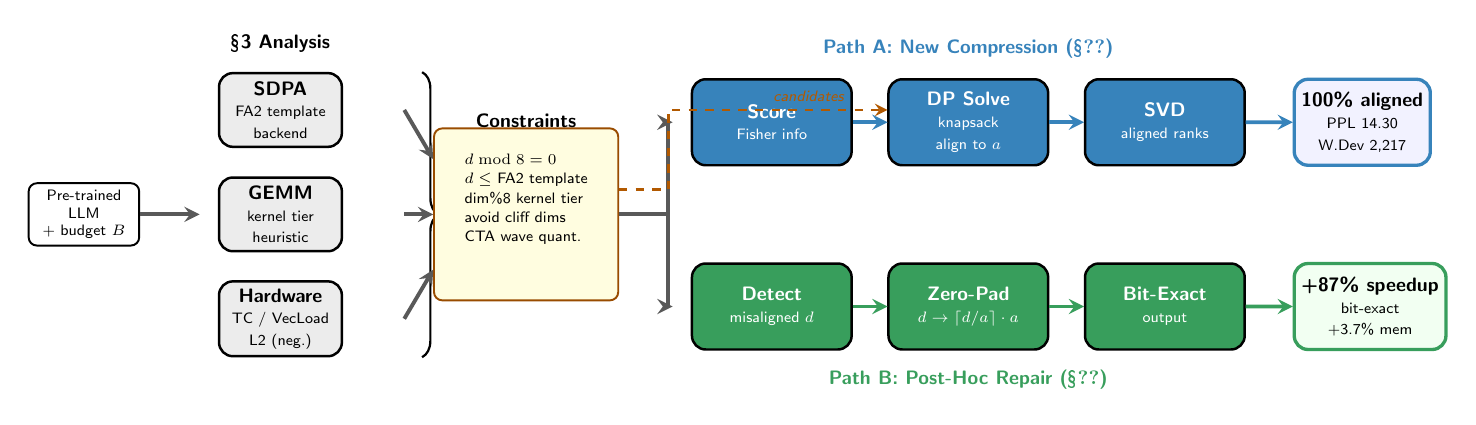
\begin{tikzpicture}[scale=0.78, every node/.style={scale=0.78},
    >=stealth,
    % Colors
    cblue/.style={fill={rgb,255:red,55;green,131;blue,187}},
    cred/.style={fill={rgb,255:red,211;green,63;blue,73}},
    cgreen/.style={fill={rgb,255:red,56;green,158;blue,92}},
    corange/.style={fill={rgb,255:red,230;green,159;blue,0}},
    cgray/.style={fill=gray!15},
    % Box styles
    phase/.style={draw, rounded corners=5pt, minimum width=2.4cm, minimum height=1.6cm,
                  line width=0.9pt, text=white, font=\sffamily\small, align=center},
    constraint/.style={draw, rounded corners=3pt, minimum width=2.0cm, minimum height=0.7cm,
                       line width=0.7pt, font=\sffamily\scriptsize, align=center,
                       fill=yellow!12, draw=orange!60!black},
    result/.style={draw, rounded corners=5pt, minimum width=2.2cm, minimum height=1.6cm,
                   line width=1.2pt, font=\sffamily\small, align=center},
    lbl/.style={font=\sffamily\small, align=center},
    arrow/.style={->, line width=1.4pt, color=gray!70!black},
    dasharrow/.style={->, line width=1.0pt, dashed, color=gray!50},
  ]

  % ===== LEFT: Analysis (§3) =====
  \node[phase, cgray, text=black, minimum width=2.0cm, minimum height=1.2cm]
    (sdpa) at (0, 1.2) {\textbf{SDPA}\\[-1pt]{\scriptsize FA2 template}\\[-1pt]{\scriptsize backend}};
  \node[phase, cgray, text=black, minimum width=2.0cm, minimum height=1.2cm]
    (gemm) at (0, -0.5) {\textbf{GEMM}\\[-1pt]{\scriptsize kernel tier}\\[-1pt]{\scriptsize heuristic}};
  \node[phase, cgray, text=black, minimum width=2.0cm, minimum height=1.2cm]
    (hw) at (0, -2.2) {\textbf{Hardware}\\[-1pt]{\scriptsize TC / VecLoad}\\[-1pt]{\scriptsize L2 (neg.)}};

  % Brace for analysis
  \node[above=0.15cm of sdpa, font=\sffamily\bfseries\small] {\S3 Analysis};
  \draw[decorate, decoration={brace, amplitude=6pt, raise=2pt}, line width=0.8pt]
    ([xshift=1.2cm]sdpa.north east) -- ([xshift=1.2cm]hw.south east);

  % ===== CENTER: Constraints =====
  \node[constraint, minimum width=3.0cm, minimum height=2.8cm]
    (constraints) at (4.0, -0.5) {};
  \node[above=-0.1cm of constraints.north, font=\sffamily\bfseries\small] {Constraints};
  \node[font=\sffamily\scriptsize, align=left, anchor=north] at ([yshift=-0.3cm]constraints.north) {
    $d \bmod 8 = 0$\\[1pt]
    $d \leq$ FA2 template\\[1pt]
    dim\%8 kernel tier\\[1pt]
    avoid cliff dims\\[1pt]
    CTA wave quant.
  };

  % Arrows: analysis → constraints
  \draw[arrow] ([xshift=1.0cm]sdpa.east) -- ([yshift=0.9cm]constraints.west);
  \draw[arrow] ([xshift=1.0cm]gemm.east) -- (constraints.west);
  \draw[arrow] ([xshift=1.0cm]hw.east) -- ([yshift=-0.9cm]constraints.west);

  % ===== RIGHT: Two paths =====
  % Path A: GAC DP (new compression)
  \node[phase, cblue, minimum width=2.6cm, minimum height=1.4cm]
    (score) at (8.0, 1.0) {\textbf{Score}\\[-1pt]{\scriptsize Fisher info}};
  \node[phase, cblue, minimum width=2.6cm, minimum height=1.4cm]
    (dp) at (11.2, 1.0) {\textbf{DP Solve}\\[-1pt]{\scriptsize knapsack}\\[-1pt]{\scriptsize align to $a$}};
  \node[phase, cblue, minimum width=2.6cm, minimum height=1.4cm]
    (svd) at (14.4, 1.0) {\textbf{SVD}\\[-1pt]{\scriptsize aligned ranks}};

  % Path B: Dimension Repair (existing model)
  \node[phase, cgreen, minimum width=2.6cm, minimum height=1.4cm]
    (detect) at (8.0, -2.0) {\textbf{Detect}\\[-1pt]{\scriptsize misaligned $d$}};
  \node[phase, cgreen, minimum width=2.6cm, minimum height=1.4cm]
    (pad) at (11.2, -2.0) {\textbf{Zero-Pad}\\[-1pt]{\scriptsize $d \to \lceil d/a\rceil \cdot a$}};
  \node[phase, cgreen, minimum width=2.6cm, minimum height=1.4cm]
    (exact) at (14.4, -2.0) {\textbf{Bit-Exact}\\[-1pt]{\scriptsize output}};

  % Arrows within paths
  \draw[arrow, color={rgb,255:red,55;green,131;blue,187}] (score) -- (dp);
  \draw[arrow, color={rgb,255:red,55;green,131;blue,187}] (dp) -- (svd);
  \draw[arrow, color={rgb,255:red,56;green,158;blue,92}] (detect) -- (pad);
  \draw[arrow, color={rgb,255:red,56;green,158;blue,92}] (pad) -- (exact);

  % Constraints → paths
  \draw[arrow] (constraints.east) -- ++(0.8,0) |- ([xshift=-0.3cm]score.west)
    node[pos=0.25, above, font=\sffamily\scriptsize\itshape] {};
  \draw[arrow] (constraints.east) -- ++(0.8,0) |- ([xshift=-0.3cm]detect.west);

  % Constraints feeds into DP
  \draw[dasharrow, color=orange!70!black]
    ([yshift=0.4cm]constraints.east) -- ++(0.8,0) |- ([yshift=0.2cm]dp.west)
    node[pos=0.82, above, font=\sffamily\scriptsize\itshape, text=orange!70!black] {candidates};

  % Path labels
  \node[above=0.15cm of dp, font=\sffamily\bfseries\small, text={rgb,255:red,55;green,131;blue,187}]
    {Path A: New Compression (\S\ref{sec:gac})};
  \node[below=0.15cm of pad, font=\sffamily\bfseries\small, text={rgb,255:red,56;green,158;blue,92}]
    {Path B: Post-Hoc Repair (\S\ref{sec:repair})};

  % Results on the right
  \node[result, fill=blue!5, draw={rgb,255:red,55;green,131;blue,187},
        right=0.6cm of svd, minimum height=1.4cm] (resA) {
    {\small\bfseries 100\% aligned}\\[-1pt]
    {\scriptsize PPL 14.30}\\[-1pt]
    {\scriptsize W.Dev 2{,}217}
  };
  \node[result, fill=green!5, draw={rgb,255:red,56;green,158;blue,92},
        right=0.6cm of exact, minimum height=1.4cm] (resB) {
    {\small\bfseries +87\% speedup}\\[-1pt]
    {\scriptsize bit-exact}\\[-1pt]
    {\scriptsize +3.7\% mem}
  };
  \draw[arrow, color={rgb,255:red,55;green,131;blue,187}] (svd) -- (resA);
  \draw[arrow, color={rgb,255:red,56;green,158;blue,92}] (exact) -- (resB);

  % Input on the left
  \node[draw, rounded corners=3pt, fill=white, line width=0.7pt,
        font=\sffamily\scriptsize, align=center, minimum width=1.8cm]
    (input) at (-3.2, -0.5) {Pre-trained\\LLM\\+ budget $B$};
  \draw[arrow] (input) -- ([xshift=-0.3cm]gemm.west |- input);

\end{tikzpicture}
\caption{\textbf{GAC framework overview.}
Analysis (\S\ref{sec:analysis}) extracts alignment constraints from three layers (SDPA, GEMM, hardware).
These constraints drive two complementary solutions:
\emph{Path~A}---alignment-aware rank allocation via multi-choice knapsack DP for new compression;
\emph{Path~B}---zero-padding repair for already-compressed models.
Both paths produce fully-aligned dimensions with no accuracy loss (DP) or bit-exact output preservation (repair).}
\label{fig:gac_framework}
\end{figure*}

\begin{figure*}[t]
\centering
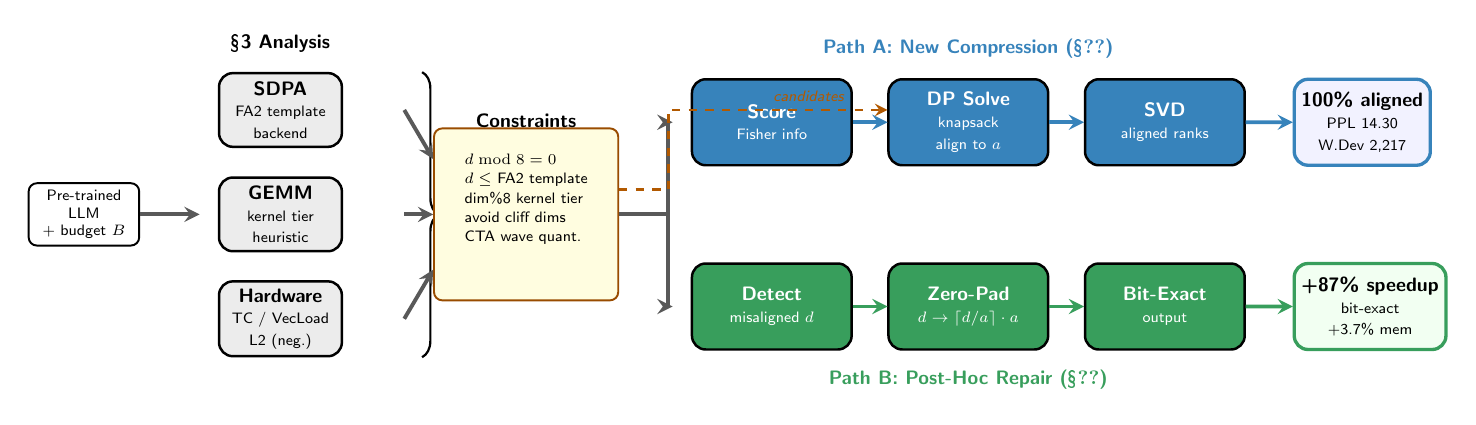
\begin{tikzpicture}[scale=0.78, every node/.style={scale=0.78},
    >=stealth,
    % Colors
    cblue/.style={fill={rgb,255:red,55;green,131;blue,187}},
    cred/.style={fill={rgb,255:red,211;green,63;blue,73}},
    cgreen/.style={fill={rgb,255:red,56;green,158;blue,92}},
    corange/.style={fill={rgb,255:red,230;green,159;blue,0}},
    cgray/.style={fill=gray!15},
    % Box styles
    phase/.style={draw, rounded corners=5pt, minimum width=2.4cm, minimum height=1.6cm,
                  line width=0.9pt, text=white, font=\sffamily\small, align=center},
    constraint/.style={draw, rounded corners=3pt, minimum width=2.0cm, minimum height=0.7cm,
                       line width=0.7pt, font=\sffamily\scriptsize, align=center,
                       fill=yellow!12, draw=orange!60!black},
    result/.style={draw, rounded corners=5pt, minimum width=2.2cm, minimum height=1.6cm,
                   line width=1.2pt, font=\sffamily\small, align=center},
    lbl/.style={font=\sffamily\small, align=center},
    arrow/.style={->, line width=1.4pt, color=gray!70!black},
    dasharrow/.style={->, line width=1.0pt, dashed, color=gray!50},
  ]

  % ===== LEFT: Analysis (§3) =====
  \node[phase, cgray, text=black, minimum width=2.0cm, minimum height=1.2cm]
    (sdpa) at (0, 1.2) {\textbf{SDPA}\\[-1pt]{\scriptsize FA2 template}\\[-1pt]{\scriptsize backend}};
  \node[phase, cgray, text=black, minimum width=2.0cm, minimum height=1.2cm]
    (gemm) at (0, -0.5) {\textbf{GEMM}\\[-1pt]{\scriptsize kernel tier}\\[-1pt]{\scriptsize heuristic}};
  \node[phase, cgray, text=black, minimum width=2.0cm, minimum height=1.2cm]
    (hw) at (0, -2.2) {\textbf{Hardware}\\[-1pt]{\scriptsize TC / VecLoad}\\[-1pt]{\scriptsize L2 (neg.)}};

  % Brace for analysis
  \node[above=0.15cm of sdpa, font=\sffamily\bfseries\small] {\S3 Analysis};
  \draw[decorate, decoration={brace, amplitude=6pt, raise=2pt}, line width=0.8pt]
    ([xshift=1.2cm]sdpa.north east) -- ([xshift=1.2cm]hw.south east);

  % ===== CENTER: Constraints =====
  \node[constraint, minimum width=3.0cm, minimum height=2.8cm]
    (constraints) at (4.0, -0.5) {};
  \node[above=-0.1cm of constraints.north, font=\sffamily\bfseries\small] {Constraints};
  \node[font=\sffamily\scriptsize, align=left, anchor=north] at ([yshift=-0.3cm]constraints.north) {
    $d \bmod 8 = 0$\\[1pt]
    $d \leq$ FA2 template\\[1pt]
    dim\%8 kernel tier\\[1pt]
    avoid cliff dims\\[1pt]
    CTA wave quant.
  };

  % Arrows: analysis → constraints
  \draw[arrow] ([xshift=1.0cm]sdpa.east) -- ([yshift=0.9cm]constraints.west);
  \draw[arrow] ([xshift=1.0cm]gemm.east) -- (constraints.west);
  \draw[arrow] ([xshift=1.0cm]hw.east) -- ([yshift=-0.9cm]constraints.west);

  % ===== RIGHT: Two paths =====
  % Path A: GAC DP (new compression)
  \node[phase, cblue, minimum width=2.6cm, minimum height=1.4cm]
    (score) at (8.0, 1.0) {\textbf{Score}\\[-1pt]{\scriptsize Fisher info}};
  \node[phase, cblue, minimum width=2.6cm, minimum height=1.4cm]
    (dp) at (11.2, 1.0) {\textbf{DP Solve}\\[-1pt]{\scriptsize knapsack}\\[-1pt]{\scriptsize align to $a$}};
  \node[phase, cblue, minimum width=2.6cm, minimum height=1.4cm]
    (svd) at (14.4, 1.0) {\textbf{SVD}\\[-1pt]{\scriptsize aligned ranks}};

  % Path B: Dimension Repair (existing model)
  \node[phase, cgreen, minimum width=2.6cm, minimum height=1.4cm]
    (detect) at (8.0, -2.0) {\textbf{Detect}\\[-1pt]{\scriptsize misaligned $d$}};
  \node[phase, cgreen, minimum width=2.6cm, minimum height=1.4cm]
    (pad) at (11.2, -2.0) {\textbf{Zero-Pad}\\[-1pt]{\scriptsize $d \to \lceil d/a\rceil \cdot a$}};
  \node[phase, cgreen, minimum width=2.6cm, minimum height=1.4cm]
    (exact) at (14.4, -2.0) {\textbf{Bit-Exact}\\[-1pt]{\scriptsize output}};

  % Arrows within paths
  \draw[arrow, color={rgb,255:red,55;green,131;blue,187}] (score) -- (dp);
  \draw[arrow, color={rgb,255:red,55;green,131;blue,187}] (dp) -- (svd);
  \draw[arrow, color={rgb,255:red,56;green,158;blue,92}] (detect) -- (pad);
  \draw[arrow, color={rgb,255:red,56;green,158;blue,92}] (pad) -- (exact);

  % Constraints → paths
  \draw[arrow] (constraints.east) -- ++(0.8,0) |- ([xshift=-0.3cm]score.west)
    node[pos=0.25, above, font=\sffamily\scriptsize\itshape] {};
  \draw[arrow] (constraints.east) -- ++(0.8,0) |- ([xshift=-0.3cm]detect.west);

  % Constraints feeds into DP
  \draw[dasharrow, color=orange!70!black]
    ([yshift=0.4cm]constraints.east) -- ++(0.8,0) |- ([yshift=0.2cm]dp.west)
    node[pos=0.82, above, font=\sffamily\scriptsize\itshape, text=orange!70!black] {candidates};

  % Path labels
  \node[above=0.15cm of dp, font=\sffamily\bfseries\small, text={rgb,255:red,55;green,131;blue,187}]
    {Path A: New Compression (\S\ref{sec:gac})};
  \node[below=0.15cm of pad, font=\sffamily\bfseries\small, text={rgb,255:red,56;green,158;blue,92}]
    {Path B: Post-Hoc Repair (\S\ref{sec:repair})};

  % Results on the right
  \node[result, fill=blue!5, draw={rgb,255:red,55;green,131;blue,187},
        right=0.6cm of svd, minimum height=1.4cm] (resA) {
    {\small\bfseries 100\% aligned}\\[-1pt]
    {\scriptsize PPL 14.30}\\[-1pt]
    {\scriptsize W.Dev 2{,}217}
  };
  \node[result, fill=green!5, draw={rgb,255:red,56;green,158;blue,92},
        right=0.6cm of exact, minimum height=1.4cm] (resB) {
    {\small\bfseries +87\% speedup}\\[-1pt]
    {\scriptsize bit-exact}\\[-1pt]
    {\scriptsize +3.7\% mem}
  };
  \draw[arrow, color={rgb,255:red,55;green,131;blue,187}] (svd) -- (resA);
  \draw[arrow, color={rgb,255:red,56;green,158;blue,92}] (exact) -- (resB);

  % Input on the left
  \node[draw, rounded corners=3pt, fill=white, line width=0.7pt,
        font=\sffamily\scriptsize, align=center, minimum width=1.8cm]
    (input) at (-3.2, -0.5) {Pre-trained\\LLM\\+ budget $B$};
  \draw[arrow] (input) -- ([xshift=-0.3cm]gemm.west |- input);

\end{tikzpicture}
\caption{\textbf{GAC framework overview.}
Analysis (\S\ref{sec:analysis}) extracts alignment constraints from three layers (SDPA, GEMM, hardware).
These constraints drive two complementary solutions:
\emph{Path~A}---alignment-aware rank allocation via multi-choice knapsack DP for new compression;
\emph{Path~B}---zero-padding repair for already-compressed models.
Both paths produce fully-aligned dimensions with no accuracy loss (DP) or bit-exact output preservation (repair).}
\label{fig:gac_framework}
\end{figure*}

\begin{algorithm}[t]
  \caption{GAC algorithm.}
  \label{alg:gac}
  \small
  \begin{algorithmic}[1]
  \Require Model $\mathcal{M}$, compressor $\mathcal{C}$, budget $B$
  \Ensure Aligned dimensions $\{d_i\}_{i=1}^n$ with $d_i \in C_i$
  \Statex \textit{Phase 1: Misaligned Compression}
  \State Apply $\mathcal{C}(\mathcal{M})$ $\to$ misaligned dims $\{d_i^*\}$, scores $\{s_i\}$
  \State Profile GeMM/SDPA $\to$ constraints (\S\ref{sec:analysis})
  \Statex \textit{Phase 2: Candidate Generation}
  \For{each weight $i = 1, \ldots, n$}
    \State Sweep dims near $d_i^*$; measure latency
    \State $C_i \gets$ dims avoiding perf.\ cliffs
  \EndFor
  \Statex \textit{Phase 3: Multi-Choice Knapsack DP}
  \State $D[0..n][0..B] \gets -\infty$;\; $D[0][0] \gets 0$
  \For{$i = 1$ to $n$}
    \For{each $d_{ij} \in C_i$}
      \State $v_{ij} \gets s_i \cdot (|W_i(d_{ij})| {-} |W_i^*|)$;\; $w_{ij} \gets |W_i(d_{ij})|$
      \For{$b = w_{ij}$ to $B$}
        \State $D[i][b] \gets \max\!\bigl(D[i][b],\; D[i{-}1][b{-}w_{ij}] + v_{ij}\bigr)$
      \EndFor
    \EndFor
  \EndFor
  \State Backtrack from $\arg\max_b D[n][b]$
  \State \Return $\{d_i\}$
  \end{algorithmic}
  \end{algorithm}
  
To bridge the gap between compression and alignment, we propose \textbf{GAC} (GPU-Aligned Compression), a paradigm that makes budget allocation system-aware so fewer parameters translate into real speedup.
GAC wraps any dimension-reducing compressor with a post-processing step, re-selecting dimensions to satisfy alignment constraint.
Given a model $\mathcal{M}$ with $n$ compressible weights $\mathcal{W}$, a compressor $\mathcal{C}$, and a parameter budget $B {=} (1{-}\rho)\,|\mathcal{W}|$ ($\rho$: compression ratio), GAC produces a fully aligned model in three steps
(Figure~\ref{fig:gac_framework}; Algorithm~\ref{alg:gac}).

\subsection{Step 1: Misaligned Compression}
\label{sec:step1}

We first apply $\mathcal{C}$ to $\mathcal{M}$ without alignment constraints.
$\mathcal{C}$ can be any established dimension-reducing compressor---e.g., ASVD~\cite{asvd} (SVD factorization) or LLM-Pruner~\cite{llmpruner} (structured pruning).
Internally, $\mathcal{C}$ computes a per-weight importance score $s_i$ using one of the proxies in Table~\ref{tab:importance_scores} (e.g., activation magnitude for ASVD, gradient-based Taylor expansion for LLM-Pruner), then allocates dimensions $\{d_i^*\}$ proportionally: higher $s_i$ retains a larger $d_i^*$.
Because $s_i$ and the resulting $\{d_i^*\}$ are continuous, the compressed model is \emph{misaligned}.

\subsection{Step 2:Dimension Sweep}
\label{sec:step2}

A na\"ive fix would round every $d_i^*$ to the nearest sweetpoint (e.g. multiple of) from the Constraints Table~\ref{tab:constraints}.
However, we cannot hard-code alignment rounding rules because different operators exhibit different behavior across different platforms (e.g., GPU architecture, PyTorch version).
A fixed heuristic that works on one platform may miss cliffs or exclude valid dimensions on another.

Instead, GAC selects candidates \emph{empirically}.
We use the heuristic constraints (e.g., $d \bmod 8 = 0$, $d \bmod 16 = 0$) to narrow the search space, then profile the kernel latency at each candidate near $d_i^*$ to verify it avoids performance cliffs on the \emph{actual} platform.
This produces a candidate set $C_i$.
For example, given $d_i^*{=}107.3$, the sweep yields $C_i{=}\{96, 104, 112, 128\}$: dimension 107 is excluded because it triggers a cuBLAS Tier-3 kernel (\S\ref{sec:library}), while 104 and 112 both land in Tier-1.
Because the sweep is hardware-specific, GAC adapts to different GPU architectures without manual tuning.

\subsection{Step 3: Constrained Optimization}
\label{sec:step3}

With misaligned dimensions $\{d_i^*\}$, importance scores $\{s_i\}$, and candidate sets $\{C_i\}$ in hand, we now select one aligned dimension per weight under the parameter budget.
Na\"ive rounding (e.g., round each $d_i^*$ to the nearest candidate) ignores two factors: (1)~different weights have different sensitivities, and (2)~rounding up at one weight consumes budget that could be spent elsewhere.
We therefore formulate a \emph{multi-choice knapsack} problem:
\begin{equation}
\max_{\{d_i\}} \sum_{i=1}^{n} s_i \cdot (|W_i| - |W_i^*|) \;\;\text{s.t.}\;\; \sum_{i} |W_i| \leq B,\;\; d_i \in C_i
\label{eq:gac}
\end{equation}
where $|W_i|$ is the parameter count of weight $W_i$ at dimension $d_i$, $|W_i^*|$ at the misaligned dimension $d_i^*$, and $C_i$ is the candidate set from Step~2.
The objective is \emph{asymmetric}: rounding up ($d_i > d_i^*$) preserves information (positive value), rounding down loses it (negative value), each scaled by the per-parameter importance $s_i$.
This lets high-importance weights receive more parameters while low-importance weights absorb the cost.

We solve Eq.~\ref{eq:gac} via dynamic programming.
For each candidate $d_{ij} \in C_i$, define value $v_{ij} = s_i \cdot (|W_i(d_{ij})| - |W_i^*|)$ and cost $w_{ij} = |W_i(d_{ij})|$.
The recurrence is:
\[
D[i][b] = \max_{j} \left\{ D[i{-}1][b - w_{ij}] + v_{ij} \right\}
\]
with complexity $O(n \cdot |C| \cdot B')$ where $B'$ is the quantized budget.
In practice ($n{=}224$, $|C| \approx 15$), the DP runs in under one second on CPU---negligible compared to the compression itself.



%% ===========================================
%% 5. EVALUATION
%% ===========================================
\section{Evaluation}
\label{sec:eval}

\subsection{Setup}

We evaluate on Llama-3-8B~\cite{llama3} with $\rho=15\%$ using an NVIDIA A100-80GB with PyTorch 2.9.1, CUDA 12.8, FP16.
We select two representative compressors that alter tensor dimensions in orthogonal ways:
\textbf{(1)~ASVD}~\citep{asvd}: activation-aware SVD ($W \to A \cdot B$) across all projection weights\footnote{All 32 layers $\times$ 7 projections (Q, K, V, O, gate, up, down) = 224 weights.}.
\textbf{(2)~LLM-Pruner}~\citep{llmpruner}: coupled structured pruning of MLP weights\footnote{Layers 3--31 (29/32 layers); gate\_proj as pruning root, propagating to up\_proj and down\_proj.}.
We compare the no compression \emph{baseline} with \emph{Unaligned} (original compression) and \emph{GAC}.

\subsection{Implementation}

GAC is implemented as a lightweight post-processing pass.
The dimension sweep profiles compression-sensitive kernels\footnote{In Transformers, mainly GeMM, SDPA and GeMV.} latency on the target GPU to build candidate sets (\S\ref{sec:step2}); the DP solver (\S\ref{sec:step3}) then selects aligned dimensions.
No model architecture changes, no runtime overhead, and no extra inference memory are required---GAC modifies only the dimension allocation before the final compression step.

\subsection{Preliminary Results}

Table~\ref{tab:main_results} summarizes the end-to-end comparison.

\begin{table}[t]
\centering
\caption{Preliminary results on Llama-3-8B ($\rho{=}15\%$). Measured with batch${=}1$, sequence length ${=}1024$.}
\label{tab:main_results}
\small
\setlength{\tabcolsep}{3pt}
\begin{tabular}{@{}lcrccc@{}}
\toprule
\textbf{Method} & \textbf{Align\%} & \textbf{PPL} & \textbf{PiQA} & \textbf{HSwag} & \textbf{Lat.\,(ms)} \\
\midrule
\rowcolor{gray!10} Baseline & 100\% & 6.14 & 0.80 & 0.50 & 99.6 \\
\midrule
ASVD & 5\% & 34.7 & 0.58 & 0.28 & 100.5\,{\scriptsize\textcolor{cred}{(+1\%)}} \\
ASVD (GAC) & 100\% & 31.3 & 0.57 & 0.26 & 67.1\,{\scriptsize\textcolor{cgreen}{($-$33\%)}} \\
\midrule
Pruner & 83\% & 9.88 & 0.80 & 0.49 & 137.7\,{\scriptsize\textcolor{cred}{(+38\%)}} \\
Pruner (GAC) & 100\% & 9.87 & 0.78 & 0.47 & 88.0\,{\scriptsize\textcolor{cgreen}{($-$12\%)}} \\
\bottomrule
\end{tabular}
\end{table}

\noindent \textbf{Alignment.}
ASVD's unconstrained allocation produces 95\% misaligned dimensions, while LLM-Pruner produces 17\% misaligned dimensions (it only prunes MLP, so attention weights stays aligned).
GAC brings both to 100\%, snapping every dimension to an aligned candidate via the asymmetric DP objective (Eq.~\ref{eq:gac}).

\noindent \textbf{Accuracy.}
We report perplexity (WikiText-2) and two downstream tasks (PiQA, HellaSwag; 200 samples each).
For ASVD, GAC lowers PPL from 34.7 to 31.3 because the DP rounds sensitive layers \emph{up}; downstream scores stay comparable
(PiQA 0.58$\to$0.51, HellaSwag 0.28$\to$0.26).
For LLM-Pruner, PPL is nearly identical (9.88 vs.\ 9.87) and downstream accuracy is well preserved (PiQA 0.80$\to$0.78, HellaSwag 0.49$\to$0.47), confirming that aligned re-selection does not sacrifice quality.

\noindent \textbf{Latency.}
Despite reducing parameters by 15\%, unaligned ASVD shows \emph{no speedup} (100.5\,ms vs.\ 99.6\,ms baseline)---the benefit is consumed by alignment overhead.
GAC restores a 1.5$\times$ speedup (67.1\,ms, $-$33\%).
For LLM-Pruner, even 83\% alignment still incurs +38\% latency; GAC eliminates the penalty, achieving 12\% speedup over the \emph{uncompressed} baseline.
The penalty grows with sequence length (Figure~\ref{fig:prefill_scaling}): from +19\% at $S{=}128$ to +38\% at $S{=}1024$, as longer sequences push GeMMs deeper into the compute-bound regime where alignment (\S\ref{sec:hardware}) dominates.

\begin{figure}[t]
\centering
\includegraphics[width=\columnwidth]{figures/fig_prefill_scaling.pdf}
\caption{Llama-3-8B latency across sequence lengths.}
\label{fig:prefill_scaling}
\end{figure}


%% ===========================================
%% 6. RELATED WORK AND DISCUSSION
%% ===========================================
\section{Related Work and Discussion}
\label{sec:related}

\textbf{LLM compression.}
SVD-based methods~\cite{asvd,svdllm2024,palu,fwsvd2022,gfwsvd2025} allocate per-layer dimensions via importance scores, producing irregular dimensions as a by-product.
Structured pruning~\cite{sparsegpt,wanda,llmpruner} and KV cache compression~\cite{h2o,quest,pyramidkv} similarly alter tensor shapes without considering hardware alignment.
Quantization~\cite{gptq,awq} preserves dimensions via fixed-width groups, naturally avoiding misalignment.
All dimension-altering compressors are \emph{hardware-agnostic}: they optimize accuracy under a size budget but ignore how chosen dimensions interact with the GPU execution stack (\S\ref{sec:analysis}).
GAC is complementary---it post-processes any such compressor's output to restore alignment.

\textbf{Hardware-aware optimization.}
HALP~\cite{halp2021} formulates CNN pruning as latency-budgeted optimization using end-to-end timing; HALOC~\cite{haloc2023} uses a differentiable latency predictor for CNN low-rank compression.
Both treat latency as a \emph{black-box} signal---they optimize aggregate runtime without isolating \emph{why} certain dimensions are slow, are tied to specific architectures, and offer no parameter-budget guarantee.
GAC instead identifies root causes (framework dispatch, kernel selection, and hardware tile alignment; \S\ref{sec:analysis}) and constrains the search space directly, guaranteeing both alignment and the parameter budget.

\textbf{Serving-side mitigations.}
Serving systems handle misalignment \emph{reactively}.
FlashAttention-2 pads to the next template (${\sim}$30\% overhead); vLLM~\cite{vllm} rejects unsupported head dimensions; TensorRT~\cite{tensorrt} pads at runtime.
These add overhead but cannot change the model.
GAC prevents misalignment at \emph{compression time}, eliminating runtime workarounds.

\textbf{Limitations and future work.}
Our evaluation covers two compressors, one model (Llama-3-8B), and one GPU (A100).
Alignment constraints grow stricter across GPU generations~\cite{nvidia_tensor_core_evolution2024}: Hopper introduces TMA with 128-byte transfers~\cite{nvidia_hopper_whitepaper}, and FlashAttention-3~\cite{flashattention3} drops support for \texttt{head\_dim} 96 and 112---suggesting that misalignment penalties will only increase on newer hardware.
Integrating GAC directly into compression libraries, extending to composed techniques (e.g., SVD + quantization), and adding a lightweight post-GAC finetuning pass are natural next steps.


%% ===========================================
%% REFERENCES
%% ===========================================
\clearpage
\bibliographystyle{ACM-Reference-Format}
\bibliography{references}


%% ===========================================
%% APPENDIX
%% ===========================================
\appendix

\section{FA2 Template Tiers and Dimension Sweep}
\label{app:fa2_templates}

We sweep \texttt{head\_dim} from 64 to 256 with $B{=}4$, $S{=}2048$, $H{=}32$.
FlashAttention-2 selects the smallest template $t \geq d$; tile width $B_c$ halves at boundaries (e.g., $128 \to 64 \to 32$), so crossing $d{=}128 \to 129$ causes $\sim$90\% latency increase.
Non-8-aligned dimensions trigger the MATH fallback (e.g., $d{=}107$ incurs 2.14\,ms, +40\% vs $d{=}112$ at 1.53\,ms on Flash).
Table~\ref{tab:fa2_templates} quantifies the tiers.

\begin{table}[h]
\centering
\caption{FA2 template tiers and performance ($B{=}4$, $S{=}2048$, $H{=}32$).}
\label{tab:fa2_templates}
\small
\setlength{\tabcolsep}{3pt}
\begin{tabular}{@{}llrrr@{}}
\toprule
Region & Template & $B_r \times B_c$ & Latency & vs.\ $t{=}64$ \\
\midrule
$d{=}64$ & 64 & 128$\times$128 & 0.74\,ms & 1.0$\times$ \\
$d \in (64,96]$ & 96 & 128$\times$64 & 1.12\,ms & 1.5$\times$ \\
$d \in (96,128]$ & 128 & 128$\times$64 & 1.47\,ms & 2.0$\times$ \\
$d \in (128,160]$ & 160 & 128$\times$32 & 2.00\,ms & 2.7$\times$ \\
$d \in (160,256]$ & 192--256 & 128$\times$32 & 2.3--2.9\,ms & 3--4$\times$ \\
\bottomrule
\end{tabular}
\end{table}

\section{GeMV Alignment Sweep}
\label{app:gemv}

Figure~\ref{fig:gemv_alignment} shows GeMV latency ($M{=}1$) with stride-1 sweeps near 4096 for $K$ and $N$.
The alignment penalty is smaller than GeMM (${\sim}$12\% on $K$, ${\sim}$4\% on $N$), consistent with GeMV being memory-bound.

\begin{figure*}[h]
\centering
\includegraphics[width=0.85\textwidth]{figures/fig_gemv_alignment.pdf}
\caption{GeMV latency ($M{=}1$, stride-1 sweep near 4096).}
\label{fig:gemv_alignment}
\end{figure*}

\section{Dimension Distribution of Evaluated Methods}
\label{app:dims}

Figure~\ref{fig:dim_distribution} shows per-layer dimension distributions for ASVD (224 projections) and LLM-Pruner (28 pruned MLP layers).
ASVD dimensions range from 300 to 3,185 with 0\% initial alignment; LLM-Pruner from 5,931 to 14,336 with 83\% alignment.

\begin{figure*}[h]
\centering
\includegraphics[width=0.85\textwidth]{figures/fig_dim_distribution.pdf}
\caption{Per-layer dimension distributions for ASVD (top) and LLM-Pruner (bottom).}
\label{fig:dim_distribution}
\end{figure*}


\section{SVD Rank Distribution Across Compression Ratios}
\label{app:scatter_ratios}

The misalignment problem persists across different compression ratios.
Figure~\ref{fig:scatter_ratios} shows dimension scatter plots for Llama-3-8B under unconstrained SVD allocation at five compression levels ($\rho=0.5$, 0.6, 0.7, 0.8, 0.9) using Fisher importance scores.
At every ratio, a substantial fraction (40--80\%) of dimensions are misaligned, confirming that dimensional misalignment is inherent to importance-based rank allocation, not an artifact of aggressive compression.

\begin{figure*}[h]
\centering
\begin{subfigure}[t]{\textwidth}
\includegraphics[width=\textwidth]{figures/scatter_1x4_meta_llama_3_8b_instruct_r0.5.pdf}
\caption{Llama-3-8B, $r$=0.5 (50\% compression)}
\end{subfigure}

\vspace{4pt}
\begin{subfigure}[t]{\textwidth}
\includegraphics[width=\textwidth]{figures/scatter_1x4_meta_llama_3_8b_instruct_r0.7.pdf}
\caption{Llama-3-8B, $r$=0.7 (30\% compression)}
\end{subfigure}

\vspace{4pt}
\begin{subfigure}[t]{\textwidth}
\includegraphics[width=\textwidth]{figures/scatter_1x4_meta_llama_3_8b_instruct_r0.9.pdf}
\caption{Llama-3-8B, $r$=0.9 (10\% compression)}
\end{subfigure}

\vspace{4pt}
\begin{subfigure}[t]{\textwidth}
\includegraphics[width=\textwidth]{figures/scatter_1x4_mistral_7b_v0_3_r0.8.pdf}
\caption{Mistral-7B, $\rho=0.8$ (cross-model)}
\end{subfigure}
\caption{SVD rank distributions across compression ratios and models.}
\label{fig:scatter_ratios}
\end{figure*}

\end{document}
